% ------------------------------------------------------------------------------------------------ %
% GRUNDLAGEN
% ------------------------------------------------------------------------------------------------ %


\section{Grundlagen}

\begin{definition}[Stichprobe]
Die Gesamtheit der Beobachtungen $x_1, \ldots, x_n$ oder der Zufallsvariablen $X_1, \ldots, X_n$ wird \emph{Stichprobe} genannt; die Anzahl $n$ heisst \emph{Stichprobenumfang}.
\end{definition}

\begin{definition}[Empirische Verteilungsfunktion]
Die \emph{empirische Verteilungsfunktion} $F_n$ zu den Messdaten $x_1,\ldots,x_n$ ist definiert durch
$$
F_n(y) := \frac{1}{n} \lvert\{x_i\mid x_i \leq y\}\rvert = \frac{1}{n} \sum_{i\text{ mit } x_i \leq y} f_i.
$$
\end{definition}

\begin{definition}[Empirischer Mittelwert]
$$
\overline{x}_n = \overline{x} = \frac{1}{n} \sum_{i=1}^n x_i
$$
\end{definition}

\begin{definition}[Empirische Varianz und Standardabweichung]
$$
s_n^2 = s^2 = \frac{1}{n-1} \sum_{i=1}^n (x_i-\overline{x})^2
$$
\end{definition}

\begin{definition}[Empirisches Quantil] Das \emph{empirische $\alpha$-Quantil} zu den geordneten Daten $x_{(1)}, \ldots, x_{(n)}$ ist gegeben durch
$$
(1-\alpha) x_{(k)} + \alpha x_{(k+1)} = x_{(k)} + \alpha \left(x_{(k+1)} - x_{(k)} \right),
$$
wobei $k = \lfloor \alpha n \rfloor$ und $\alpha \in (0,1)$.
Damit liegt etwa der Anteil $\alpha$ unterhalb des empirischen $\alpha$-Quantils, und somit etwa der Anteil $1-\alpha$ oberhalb.
\end{definition}

\begin{definition}[Empirischer Median]
Der \emph{empirische Median} ist definiert als das $0.5$-Quantil.
\end{definition}


% ------------------------------------------------------------------------------------------------ %
% DESKRIPTIVE STATISTIK
% ------------------------------------------------------------------------------------------------ %


\section{Deskriptive Statistik}


% ------------------------------------------------------------------------------------------------ %
% HISTOGRAMM
% ------------------------------------------------------------------------------------------------ %


\subsection{Histogramm}

Bei grossem Stichprobenumfang $n$ werden benachbarte Werte zu einer Klasse zusammengefasst. Der Wertebereich der Daten wird dadurch in disjunkte Intervalle (die Klassen) unterteilt.
\begin{compactenum}[i)]
\item Die Anzahl der Klassen sollte von der Gr�ssenordnung $\sqrt{n}$ sein.
\item Die Klassenbreite sollte f�r alle Klassen gleich sein; als Ausnahme k�nnen die Klassen am linken und rechten Rand gr�sser sein (Ausreisser).
\end{compactenum}

\begin{figure}[htb]
\begin{center}
\scalebox{0.6}[0.6]{
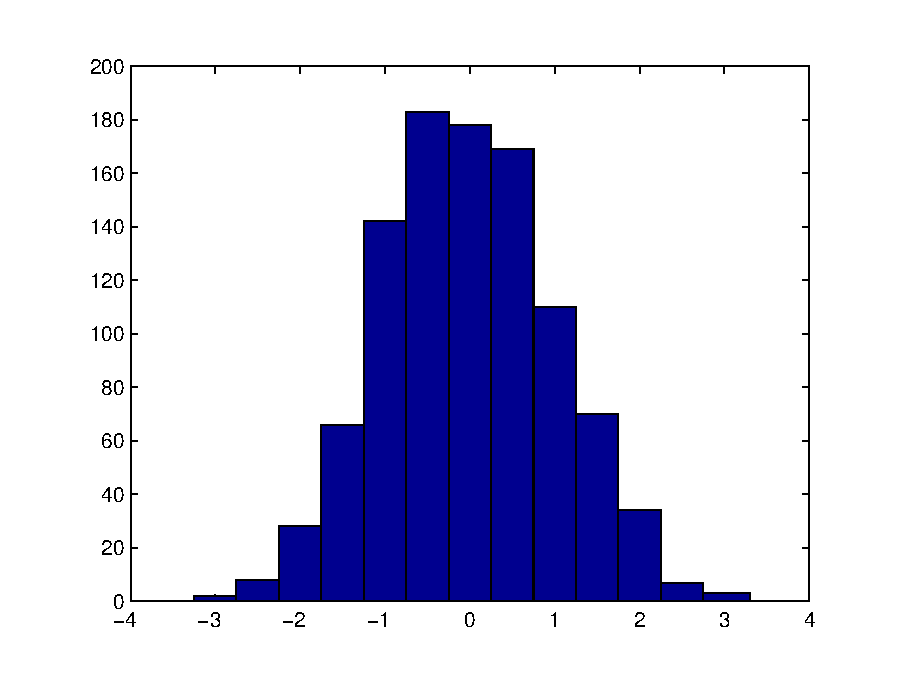
\includegraphics{figures/hist.eps}}
\end{center}
\vspace{-2em}
\caption{Histogramm einer standard-norvmalverteilten Zufallsvariable.}
\end{figure}


% ------------------------------------------------------------------------------------------------ %
% BOXPLOT
% ------------------------------------------------------------------------------------------------ %


\subsection{Boxplot}

Aus einem Boxplot l�sst sich folgendes ablesen:
\begin{compactenum}[a:]
\item empirischer Median
\item empirisches $0.25$-Quantil
\item empirisches $0.75$-Quantil
\item kleinster Datenwert $x_i$ mit $b-x_i < 1.5 (c-b)$
\item gr�sster Datenwert $x_i$ mit $x_i - c < 1.5 (c-b)$
\item Ausreisser
\end{compactenum}

\begin{figure}[htb]
\begin{center}
\scalebox{0.6}[0.6]{
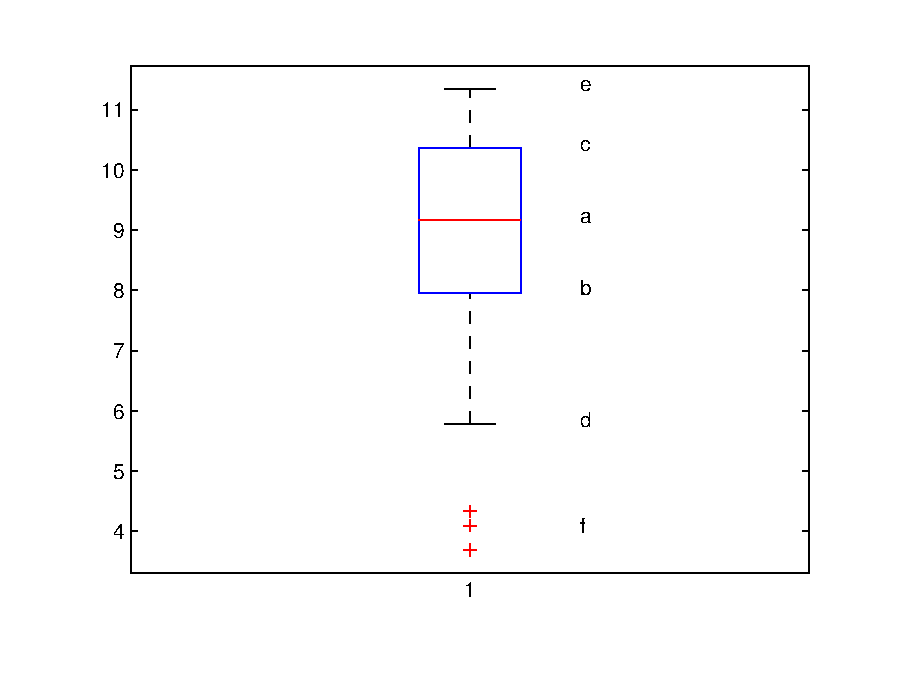
\includegraphics{figures/boxplot.eps}}
\end{center}
\vspace{-3em}
\caption{Boxplot}
\end{figure}
%a: empirischer Median, b: empirisches $0.25$-Quantil, c: empirisches $0.75$-Quantil, d: kleinster Datenwert $x_i$ mit $b-x_i < 1.5 (c-b)$, e: gr�sster Datenwert $x_i$ mit $x_i - c < 1.5 (c-b)$.


% ------------------------------------------------------------------------------------------------ %
% QQ-PLOT
% ------------------------------------------------------------------------------------------------ %


\subsection{QQ-Plot}

Mit einem \emph{QQ-Plot} (Quantil-Quantil) kann man die Abweichung der Daten von einer gew�hlten Modell-Verteilung $F$ graphisch �berpr�fen.

Es werden die empirischen Quantile auf der $y$-Achse gegen�ber den theoretischen Quantilen auf der $x$-Achse geplottet.


% ------------------------------------------------------------------------------------------------ %